\chapter[Mitigating Initialisation Impact through Flat Minima: Fast Rates for Small Gradients]{Mitigating Initialisation Impact through Flat Minima: Fast Rates for Small Gradients}
\label{chap:gen-flat-minima}
\addchapterlof
\addchapterloa
\addchapterloe
 
\vspace{-2.0cm}
\begin{center}
\textbf{This chapter is based on the following paper}\\[-0.1cm]
\end{center}
\printpublication{haddouche2024pac}


\vspace{0.2cm}
\minitoc

\begin{abstract}
\vspace{-0.2cm}
In \Cref{chap:online-pb} we saw that a way to attenuate the impact of the prior, seen as an initialisation, in PAC-Bayes training is online learning, allowing the prior to evolve alongside the posterior through time. However, a legitimate question is to wonder whether the prior could be attenuated, even in the batch learning setting which is widely used in practice. Maintaining the vision of the prior as initialisation, we propose in this chapter to attenuate the impact of the prior in the batch setting through faster convergence rate. The proposed results hold when a flat minimum has been reached, \ie a minimum whose its neighbourhood nearly minimises the loss as well. Then, a sharper understanding of generalisation can be reached when exploiting the benefits of a successful optimisation process. Indeed, this study is particularly meaningful in the context of deep learning, where it has been shown that flat minimum (also known as sharpness) correlates to a good generalisation ability.  
\end{abstract}

\newpage

\section{Introduction}

Can we make the impact of the prior vanish at a faster rate than $1/\sqrt{m}$ in the context of batch learning? While this is desirable from an optimisation perspective, this is not what is proposed by classical PAC-Bayes bounds, considering all elements of $\Mcal(\Hcal)$ simultaneously. The challenge of this study is to obtain faster rates for a smaller class of posteriors. Doing so, we aim to attenuate the impact of the initialisation (seen as prior) for nonnegative heavy-tailed losses, potentially satisfying geometric assumptions such as gradient-lipschitz, making a promising step towards concrete optimisation settings. The practical way to do so is to obtain results holding only for posteriors distributions focusing on \emph{flat minima}, which can be seen, \eg in deep learning, as a benefit of a successful optimisation process.

Indeed, dating back to \citet{hochreiter1997flat}, it has been hypothesised that the notion of `flatness' (or sometimes equivalently referred to as `sharpness') has tight links with the generalisation error: among the minima (belonging to $\hat{\Risk}_{\S_m}$) that is found by the learning algorithm, the `flatter' the minimum is, the lower is the generalisation error.
While the initial flatness notion was (vaguely) defined through low Kolmogorov complexity, there is no single formal definition of `flatness'.
Hence, several flatness notions have been considered, which typically are based on the second-order derivatives of the empirical risk around the local minimum found by the algorithm, such as $\mathrm{trace}(\nabla^2 \hat{\Risk}_{\S_m}(h))$, see \eg, \citet{jastrzkebski2017three, wen2023sharpness}.


While there have been several attempts to link some form of flatness to generalisation in a mathematically rigorous way \citep{neyshabur2017explor,petzka2021relative,yue2023sharpness, andriushchenko2023modern}, mainly in the framework of `sharpness aware minimisation'~\citep{foret2020sharpness}, it has been recently shown that flat minima do not always imply good generalisation.
In fact, there exist scenarios such that the flattest minima achieve the worst generalisation performance compared to non-flat ones \citep{wen2023sharpness}. 


In this study, we aim at developing novel links between flatness and the generalisation error from a PAC-Bayesian perspective \citep[see \eg, ][]{guedj2019primer,hellstrom2023generalization,alquier2024user}.
Denoting by $\Q$, the probability distribution of the algorithm output $h$ (or the output of a learning algorithm), we identify sufficient conditions on $\Q$ such that flatness always implies good generalisation.
More precisely, we make the following contributions:
\begin{itemize}
    \item We show that, when $\Q$ satisfies the Poincaré inequality and a technical condition that we identify, we can obtain a `fast-rate' generalisation bound that diminishes with rate $\frac{1}{m}$ (rather than $\frac{1}{\sqrt{m}}$) and mainly contains two terms:  
    \begin{enumerate}[label=(\roman*)]
        \item The flatness term: $ \EE_{h\sim \Q}\LB \frac{1}{m}\sum_{i=1}^m \|\nabla_h\ell(h,\z_i)\|^2 \RB$.
        This term is directly linked to the Hessian of the loss $\ell$, due to the connection between the Fisher information and the Hessian of the loss \cite{bickel2015mathematical}.
        For instance, under certain conditions, it can be shown that $\mathrm{trace}(\nabla^2 \hat{\Risk}_{\S_m}(h)) = \frac{2}{m}\sum_{i=1}^m \|\nabla_h \ell(h,\z_i)\|^2$ \citep[Lemma 4.1]{wen2023sharpness}.  
        \item The classical PAC-Bayesian complexity term $\KL(\Q,\P)$, where $\KL$ denotes the Kullback-Leibler divergence and $\P$ is data-independent `prior' distribution. 
    \end{enumerate}
    \item We then further analyse the term $\KL(\Q,\P)$.
    We show that, when $\Q$ is a Gibbs distribution, \ie, $\Q(h)\propto \exp(- \gamma \hat{\Risk}_{\S_m}(h)) \P(h)$ for some $\gamma >0$ and $\P$ satisfies a log-Sobolev inequality, the generalisation error can be controlled \emph{solely} by the term: $\gamma^2 c_{LS}(\P)\EE_{h\sim \Q}[ \|\nabla_h \hat{\Risk}_{\S_m}(h) \|^2 ]$, where $c_{LS}(\P)$ denotes the log-Sobolev constant of the prior $\P$. 
    \item We finally go beyond the KL divergence to link flat minima to deterministic predictors (\ie, when $\Q$ is a Dirac distribution) through a novel Wasserstein-based generalisation bound for gradient Lipschitz loss functions. 
\end{itemize}
We provide a numerical assessment of the technical condition underlying our main result, suggesting that it is suitable in the case of neural networks on classification tasks, confirming the relevance of our bounds to better understand the generalisation ability of neural networks.
Our results shed further light on the impact of the flatness of the minima over the generalisation error: when the learning algorithm ensures a sufficiently regular distribution over the parameters, the generalisation error can be directly controlled by the flatness of the region found by the algorithm.  

\section{Preliminaries}

\textbf{Framework.}
We consider a predictor set $\Hcal\subseteq \mathbb{R}^d$ equipped with a norm $\|.\|$, a data space $\Zcal$ and the space of distributions over $\Hcal,\Mcal(\Hcal)$.
We also consider a loss function $\ell : \Hcal\times \Zcal \rightarrow \mathbb{R}$. 
We assume that we have access to a \iid dataset $\S=(\z_i)_{i\geq 1}\in\Zcal^\Nbb$  with associated distribution $\mathcal{D}$. For each $m\geq 1$, we define $\S_m:= \{\z_1,\cdots,\z_m\}$.
In PAC-Bayes learning, we construct a data-driven posterior distribution $\Q\in\Mcal(\Hcal)$ with respect to a prior distribution $\P$. 
To assess the generalisation ability of a predictor $h\in\Hcal$, we define  the \emph{population risk} to be $\Risk_{\D} (h) \defeq \EE_{\z\sim \mu}[\ell(h,\z)]$ and for each $m$, its empirical counterpart $\hat{\Risk}_{\S_m} (h) \defeq \frac{1}{m}\sum_{i=1}^{m} \ell(h,\z_{i})$. As PAC-Bayes focuses on elements of $\Mcal(\Hcal)$, we also define the expected risk and empirical risks for $\Q\in\Mcal(\Hcal)$ as $\Risk_{\D}(\Q):= \EE_{\h\sim Q}[ \Risk_{\D}(\h)]$ and $\hat{\Risk}_{\S_m}(\Q):= \EE_{\h\sim Q}[ \hat{\Risk}_{\S_m}(\h)]$.
PAC-Bayes bounds usually aim at controlling the \emph{expected generalisation error (or gap)} for each dataset size $m$, i.e.,  $\Delta_{\S_m}(\Q):=
\Risk_{\D}(\Q) - \hat{\Risk}_{\S_m}(\Q)$.

\paragraph{Background on Poincaré and log-Sobolev inequalities.} In this work, we exploit Poincaré and log-Sobolev inequalities in the PAC-Bayes framework.
We first recall the definition of Poincaré and log-Sobolev inequalities.
To do so, for a fixed distribution $\Q$, we define the \emph{Sobolev space of order $1$} on $\mathbb{R}^d$ as follows:
\[ \mathrm{H}^{1}(\Q) := \left\{ f\in \mathrm{L}^2(\Q)\cap \mathrm{D}_1(\mathbb{R}^d)\mid \|\nabla f\|\in \mathrm{L}^2(\Q) \right\}, \] 
where $\mathrm{D}_1(\mathbb{R}^d)$ denotes the set of derivable functions $f : \mathbb{R}^d \to \mathbb{R}$. 

\begin{definition}[Poincaré and Logarithmic Sobolev inequalites]
A measure $\Q$ satisfies a \emph{Poincaré inequality} with constant $c_{P}(\Q)$ if for all function $f\in \mathrm{H}^{1}(\Q)$ we have 
\begin{align*}
 \Var_\Q(f) \leq c_{P}(\Q) \EE_{h\sim \Q}\left[ \|\nabla f (h)\|^2 \right],
\end{align*}
where $\Var_\Q(f) = \EE_{h\sim\Q} \left[f(h) - \EE_{h\sim\Q}[f(h)]\right]^2$ is the \emph{variance} of $f$ \wrt $\Q$.
We then say that $\Q$ is Poincaré with constant $c_{P}(\Q)$, or that $\Q$ is $\Poinc(c_{P})$.
Also, $\Q$ satisfies a \emph{log-Sobolev inequality} with constant $c_{LS}(\Q)$ if for all function $f\in \mathrm{H}^{1}(\Q)$ we have 
\begin{align*}
\EE_{h\sim\Q}\LB f^2(h)\log\LP \frac{f^2(h)}{\mathbb{E}_{h\sim\Q}\LB f^2(h)\RB}\RP \RB \leq c_{LS}(\Q) \EE_{h\sim \Q}\left[ \|\nabla f (h)\|^2 \right],
\end{align*}
where the term on the left hand side is the \emph{entropy} of $f^2$, denoted as $\Ent_Q(f^2)$.
We then say that $\Q$ is log-Sobolev with constant $c_{LS}(\Q)$, or that $\Q$ is $\Lsob(c_{LS})$.
\end{definition}
The class of Gaussian distributions is an important particular case of distributions satisfying both Poincaré and log-Sobolev inequalities, this is the subject of Proposition \ref{prop:gaussian-inequalities}.
\begin{proposition}\label{prop:gaussian-inequalities}
For a given pair $(\mu,\Sigma)$ of mean and covariance matrix in $\mathbb{R}^d$, define $\Q= \Ncal(\mu, \Sigma)$.
Then we have, for any $f \in \mathrm{H}^{1}(\Q)$:
\begin{align*}
\Ent_\Q(f^2) \leq 2\mathbb{E}_{\Q}\left[ \left\langle \Sigma \nabla f, \nabla f\right\rangle \right],\;\text{and }  \Var_\Q(f^2) \leq \mathbb{E}_{\Q}\left[ \left\langle \Sigma \nabla f, \nabla f\right\rangle \right].
\end{align*}
Thus, $\Q$ is $\Lsob(c_{LS})$ with constant $c_{LS}(\Q)=2\|\Sigma\|_{op}$ and also  $\Poinc(c_{LS})$ with constant $c_{LS}(\Q)=\|\Sigma\|_{op}$, where $\|.\|_{op}$ denotes the operator norm. 
\end{proposition}
In \Cref{prop:gaussian-inequalities}, the first inequality can be derived from the classical log-Sobolev inequality for $\Ncal(\zerobf,\textrm{Id})$ stated in \citet{gross1975lsi}, with a change of variable. Similarly, the Poincaré inequality can be obtained through a change of variable from the Poincaré inequality for $\Ncal(\zerobf,\textrm{Id})$ which is a particular case of the Brascamp-Lieb inequality for log-concave probability measures \citep{brascamp1976extensions} and is stated explicitly in \citet[Theorem 1]{beckner1989new}. 


We now focus on specific posterior distributions called \emph{Gibbs posteriors, or Gibbs distributions}.
For a fixed loss $\ell$ and dataset $\S_m$, the Gibbs posterior, \wrt prior $\P\in\Mcal(\Hcal)$, risk $\hat{\Risk}_{\S_m}$ and \emph{inverse temperature} $\gamma>0$.is defined as $\P_{-\gamma \hat{\Risk}_{\S_m}}$ such that  $d\P_{-\gamma \hat{\Risk}_{\S_m}}(h)\propto \exp( - \gamma \hat{\Risk}_{\S_m}(h) ) d\P(h)$. 
Gibbs posteriors are a class of closed-form solutions for relaxation of \citet[Theorem 1.2.6]{catoni2007pac} stated, for instance, in \citet[Theorem 4.1]{alquier2016properties}. 
\Cref{prop:gibbs_logsob} shows that when the prior and the loss satisfies a few properties, then the associated Gibbs posterior is $\Lsob(c_{LS})$.

\begin{proposition}\label{prop:gibbs_logsob}
Assume that $\P$ is a probability measure on $\mathbb{R}^d$ such that $d\P(h) \propto \exp(-V(x))$ with $V$ a smooth function such that $Hess(V)\succeq \frac{2}{c_{LS}(\P)}\mathrm{Id}$.
Assume that $\ell= \ell_1 + \ell_2$ with $\ell_1$ convex, twice differentiable and $\ell_2$ bounded. 
Then for any $\gamma>0$, the Gibbs posterior $\Q= \P_{-\gamma\hat{\Risk}_{\S_m}}$ is $\Lsob(c_{LS})$ with constant $c_{LS}(\Q)= c_{LS}(\P)\exp\LP 4\|\ell_2\|_{\infty}\RP $.
\end{proposition}
\Cref{prop:gibbs_logsob} applies, \eg, when $\P$ is a Gaussian prior $\P=\Ncal(\mu_\P,\Sigma_\P)$. Notice that in this case $c_{LS}(\P)= 2\|\Sigma_\P\|_{op}$. This property is a straightforward application of \citet[Corollary 2.1]{chafai2004entropies} with \citet[Property 2.6]{guionnet2003lectures} and is stated in \Cref{sec: supp_background} for completeness.
Finally, notice that satisfying a log-Sobolev inequality is stronger than satisfying a Poincaré one. This is stated for instance in \citet[Proposition 2.1]{ledoux2006concentration} and properly recalled in \Cref{sec: supp_background}. 

\section{Reaching a flat minimum allows Poincaré posteriors to generalise well}
\label{sec:poincare_gauss}

\subsection{Fast rate PAC-Bayes bounds for heavy-tailed losses}  
\label{sec:fast_rates_gradient_h}

In order to obtain fast rates, \ie, bounds converging to zero faster than $\frac{1}{\sqrt{m}}$,  we exploit the notion of flat minimum (where the loss takes a small value in the neighbourhood of the minimum).
Indeed, in an overparametrised setting such as neural networks, it is likely to obtain such a minimum once the optimisation phase has been performed, as there are much more parameters than training data.
We exploit this flatness property within PAC-Bayes bounds through the gradient norm $\| \nabla_h \ell(.,\z)\|$ of the loss \wrt the predictor $h$ for any $\z$.
This is, to the best of our knowledge, the first attempt to do so as \citet{gat2022grad} focus on gradients with respect to the data $\nabla_{\z}\ell$ (one does not optimise on those, as the dataset is fixed in practice).
  
In this section, we consider posterior distributions $\Q$ being $\Poinc(c_P)$.
This assumption covers the important case of Gaussian measures (\Cref{prop:gaussian-inequalities}) as well as all measures satisfying a log-Sobolev inequality (\Cref{prop:ls_implies_poinc}).
We focus on PAC-Bayes bound holding for distributions $\Q$ satisfying a particular assumption involving the data distribution $\D$ (contrary to many PAC-Bayes bounds holding for all $\Q$).
We then define the \emph{error} of $\Q\in \Mcal(\Hcal)$ for any datum $\z\in\Zcal$ as $\Err(\ell,\Q,\z)\defeq \mathbb{E}_{h\sim\Q}[\ell(h,\z)]$ and identify Assumption \ref{hyp:relaxed_bounded} to later involve flat minima.

  
  \begin{assumption}
    \label{hyp:relaxed_bounded}
    We say that $\Q\in\Mcal(\Hcal)$ is \emph{quadratically self-bounded} with respect to $\ell$ and constant $C>0$ (namely $\texttt{QSB}(\ell,C)$) if
    \[ \mathbb{E}_{\z\sim \D}\LB \Err(\ell,\Q,\z)^2 \RB \leq C \Risk_\D(\Q) \LP = C\mathbb{E}_{\z\sim \D}\LB \Err(\ell,\Q,\z) \RB \RP.   \]
  \end{assumption}
Assumption \ref{hyp:relaxed_bounded} is a relaxation of boundedness, as if $\ell\in[0,C]$ then it is $\texttt{QSB}(\ell,C)$.
It is an alternative to the bounded expected variance assumption in anytime-valid PAC-Bayes bounds as in \Cref{chap: pb-ht} and \citep{chugg2023unified}.
An issue with such boundedness assumption is that it has to hold for all posteriors, including those providing poor generalisation performances.
This is avoided by the $\texttt{QSB}$ assumption which intricate the properties of $\D,\ell$ and $\Q$.
Such a design is in line with the conclusions of the recent work of \citet{gastpar2023fantastic}, inviting to derive generalisation bounds valid for specific pairs $(\Q,\D)$ (and not uniformly valid for all such pairs).
Finally, we interpret $C$ as a contraction constant attenuating, on average, the local expansion (governed by variances of $\Q$, and $\D$) of the loss around the mean of $\Q$.
Exploiting the PAC-Bayes supermartingales bounds of \Cref{chap: pb-ht} and \citet{chugg2023unified} alongside Poincaré inequality leads to the following. 

\begin{theorem}\label{th:poincaré_gauss}
For any $C>0$, any $\frac{2}{C}>\lambda >0$, any data-free prior $\P$, any  $\ell\geq 0$ and any $\delta\in [0,1]$, we have, with probability at least $1-\delta$ over the sample $\S$, for any $m>0$, any $\Q$ being $\Poinc(c_P)$, $\texttt{QSB}(\ell,C)$ and $\ell(.,\z)\in \mathrm{H}^{1}(\Q)$ for all $\z$,
\begin{multline*}
\Risk_{\D}(\Q) \leq \frac{1}{1-\frac{\lambda C}{2}} \LP \hat{\Risk}_{\S_m}(\Q) + \frac{\KL(\Q,\P) +\log(1/\delta)}{\lambda m} \RP \\
+ \frac{\lambda}{2-\lambda C} c_{P}(\Q)\EE_{\z\sim\D} \LB \EE_{h\sim \Q}\LP \|\nabla_h \ell(h,\z)\|^2 \RP \RB.
\end{multline*}
\end{theorem}
This theorem shows that, for any posterior being \texttt{QSB} \wrt the distribution $\D$, fast rates are achievable as long as $\hat{\Risk}_{\S_m}\approx 0$, and expected gradients are vanishing.
While the first condition is often involved for deep neural networks in the overparametrised setting, the second holds if a flat minimum has been reached through the optimisation process.
Then, taking $\lambda = \frac{1}{C}$ ensures an anytime-valid PAC-Bayesian bound with a fast rate of $\frac{1}{m}$.
Otherwise, for a fixed $m$, taking $\lambda= \frac{m^{-\alpha}}{C}$, $\alpha \in \LB0;\frac{1}{2}\RB$ allows to adapt the convergence speed \wrt the behaviour of the gradients. 
In the case of constant gradients, we recover a convergence rate of $\frac{1}{\sqrt{m}}$, matching \citet[Theorem 4.1]{alquier2016properties}. 

  
\noindent\textbf{On the role of flat minima in PAC-Bayes learning.} 
Theorem \ref{th:poincaré_gauss} suggests that, in order to attain good generalisation ability, the mean of $\Q$ has to be close from two minima: 
\emph{(i)} on $\hat{\Risk}_{\S_m}$ in order to make $\hat{\Risk}_{\S_m}$ small, and \emph{(ii)} on $\Ebb_{\z\sim\D}[\|\nabla_h \ell(h,\z)\|^2]$  to make the gradients small. The variance of $\Q$ has to fit the flatness of those minima, the flatter they are, the larger the variance in order to shrink the expected terms on the right-hand-side of Theorem \ref{th:poincaré_gauss}. Finally, the KL term invites, \eg for Gaussian distributions, to consider high variances, hence flat minima to maintain a small value of the bound.
  %Indeed, we interpret $C$ as a contraction constant translating the sharpness of the minimum on $\Risk_\D$:  the flatter the minimum, (\eg $\Risk_\D(\mu)= 0$), the closer  $\Risk_\D(\Q)$ from 0, then $\Risk_\D(\Q)^2$ is even smaller, allowing smaller $C$ and translating contractions of the loss. \umut{I think this paragraph is very important in terms of the meaning of the bound because flatness is in the core of the paper. Could you rewrite it by giving more intuitive details? Right now it's not very clear to me what it's meant by sharpness/flatness and how explicitly it's linked to $C$. Also there are existing "flatness" notions, how does this relate to those? }
  
\noindent\textbf{A focus on $C$.}
Taking $\lambda= \frac{1}{C}$ in Theorem \ref{th:poincaré_gauss} attenuates the impact of the prior distribution and amplifies the gradient term. Then, a small $C$ is desirable when working with flat minima to attenuate an ill-designed prior. Having a small $C$ is reachable in practice: we show in \Cref{sec: expes}, for a classification task on MNIST, that the \texttt{QSB} assumption is verified with $C$ strictly smaller than $1$ when considering neural networks.
  
\noindent\textbf{High probability bounds with fast rates, a paradox?} \citet[page 7]{grunwald2021mac} showed that, for a trivial $\Hcal=\{h\}\subset \Rbb^d$, for any loss, any \iid dataset $\S_m$ with variance $\sigma^2$, we have asymptotically, with probability at least $\alpha$, for a constant $C_{\alpha}$ depending on $\alpha$ and $\Ncal(\zerobf,\textrm{Id})$, we have $\Risk_\D(h) \geq \hat{\Risk}_{\S_m}(h) + C_{\alpha}\frac{\sigma^2}{\sqrt{m}}$. Is it paradoxical with Theorem \ref{th:poincaré_gauss}? The answer is no: the bound in \citet{grunwald2021mac} gives an asymptotic lower bound on the convergence of $\hat{\Risk}_{\S_m}(h)$ to  $\Risk_\D(h)$. Theorem 
  \ref{th:poincaré_gauss} informs us on how $\Risk_\D$ is getting closer from $\frac{1}{1-\lambda/2}\hat{\Risk}_{\S_m}$ which converges to $\frac{1}{1-\lambda/2}\Risk_\D>\Risk_\D$ as the loss is non-negative.  
  Theorem \ref{th:poincaré_gauss} then show the existence of a `transition regime' involving a fast rate. Once  $\frac{1}{1-\lambda/2} \hat{\Risk}_{\S_m}$ is reached, the clower bound of \citet{grunwald2021mac} ensures an asymptotic regime with slow convergence rate. Note that such transition regimes already appeared in the literature in \citet{tolstikhin2013pac,mhammedi2019pac} at the cost of additional variance terms compared to Theorem \ref{th:poincaré_gauss}. However, such fast rates have never been linked before to flat minima (and optimisation in general), highlighting the potential of our bound to explain the ability of deep neural networks to generalise well in the overparametrised setting ($m$ far smaller than the dimension of $\Hcal$), where flat minima are likely to be reached, as studied, \eg, in \citet{dziugaite2020search}, showing correlations between flat minima and generalisation for various learning problems. 

  \begin{proof}[of Theorem \ref{th:poincaré_gauss}]
We start from \citet[Corollary 17]{chugg2023unified} instantiated with a single $\lambda$, \iid data and a prior $\P$. 
With probability at least $1-\delta$, for any $\Q\in\Mcal(\Hcal)$ and $m>0$:
\begin{align*}
\Risk_{\D}(\Q) \leq  \hat{\Risk}_{\S_m}(\Q) + \frac{\KL(\Q,\P) +\log(1/\delta)}{\lambda m} 
+ \frac{\lambda }{2}\left(   \EE_{h\sim \Q}\left[\mathbb{E}_{\z\sim \D}[\ell (h,\z)^2]  \right]  \right),
\end{align*} 
where $\z\sim \D$ is independent of $\S$. 
We study the last term on the right-hand side. First, applying Fubini's theorem gives: 
\begin{align*}
\EE_{h\sim \Q}\left[\mathbb{E}_{\z\sim \D}[\ell (h,\z)^2] \right] & = \mathbb{E}_{\z\sim \D}\left[ \EE_{h\sim \Q}[\ell (h,\z)^2] \right] \\
& = \EE_{\z\sim\D} \LB \Var_{h\sim \Q}\LP \ell(h,\z) \RP + \LP \EE_{h\sim\Q}[\ell(h,\z)] \RP^2 \RB .
\intertext{As for any $\z$, $\ell(.,\z)\in \mathrm{H}^{1}$, we apply Poincaré's inequality to obtain: }
& \leq  \EE_{\z\sim\D} \LB c_{P}(\Q)\EE_{h\sim \Q}\LP \|\nabla_h \ell(h,\z)\|^2 \RP + \LP \EE_{h\sim\Q}[\ell(h,\z)] \RP^2 \RB  .
\end{align*}
Using that $\Q$ is $\texttt{QSB}(\ell,C)$ and re-organising the terms gives: 
\begin{multline*}
\Risk_{\D}(\Q) \leq \frac{1}{1-\frac{\lambda C}{2}} \LP \hat{\Risk}_{\S_m}(\Q) + \frac{\KL(\Q,\P) +\log(1/\delta)}{\lambda m} \RP \\
+ \frac{\lambda}{2-\lambda C} c_{P}(\Q)\EE_{\z\sim\D} \LB \EE_{h\sim \Q}\LP \|\nabla_h \ell(h,\z)\|^2 \RP \RB. 
\end{multline*}
\end{proof}
\noindent{}It is possible to go beyond the $\texttt{QSB}$ assumption.
This comes at the cost of an upper bound on $\Risk_\D$ as well as a supplementary Poincaré assumption on $\D$.  

\begin{corollary}\label{cor:poincaré_pacb}
For any $C>0$, any $\delta\in (0,1)$ any $\frac{2}{C}>\lambda >0$, any data-free prior $\P$, any $\ell\geq 0$ such that, for any $\z\in\Zcal$, we have $\ell(.,\z)\in \mathrm{H}^{1}$ and for any $h$, the loss function $\ell(h,.)$ is $\Ccal^1$ almost everywhere on $\Zcal$.
If the data distribution $\D$ is $\Poinc(c_P)$, then with probability at least $1-\delta$ over the sample $\S$, for any $m>0$, any posterior $\Q$ being $\Poinc(c_P)$ with $\Risk_\D(\Q)\leq C$:

\begin{multline*}
\Risk_{\D}(\Q) \leq \frac{1}{1-\frac{\lambda C}{2}}\LP \hat{\Risk}_{\S_m}(\Q) + \frac{\KL(\Q,\P) +\log(1/\delta)}{\lambda m}\RP \\
+ \frac{\lambda}{2-\lambda C}\LP c_{P}(\Q)\EE_{\z\sim\D} \LB \EE_{h\sim \Q}\LP \|\nabla_h \ell(h,\z)\|^2 \RP \RB  + c_{P}(\D)\EE_{\z\sim\D} \LP \LM\EE_{h\sim\Q}[\nabla_z \ell(h,\z)] \RM^2\RP  \RP.
\end{multline*}     
\end{corollary}   
Proof is deferred to Section \ref{sec:proof_poincaré_pacb}.
Corollary \ref{cor:poincaré_pacb} states that, if $\Q$ reached a flat minimum (meaning $\|\nabla_h\ell\|$ is small), and this minimum is robust to the training dataset (meaning $\|\nabla_\z\ell\|$ is small), then a fast rate is attainable while only requiring an upper bound on $\Risk_\D(\Q)$.
This conclusion holds when $\D$ \Poinc, encompassing the case of Gaussian mixtures \citep{schlichting2019poinc}, which can approximate any smooth density \citep[as recalled in][]{gat2022grad}.
However, the Poincaré constant of a general mixture is not known, and the upper bound of \citet{schlichting2019poinc} scales with the number of components, involving potentially high $\chi^2$ divergences.\\

\noindent\textbf{Comparison with \citet{gat2022grad}}. We compare Corollary \ref{cor:poincaré_pacb} with \citet[Theorems 3.5, 3.6]{gat2022grad}.
First, our result holds with the assumption that $\D$ follows a Poincaré inequality, which is strictly less restrictive than assuming a log-Sobolev inequality (Proposition \ref{prop:ls_implies_poinc}).
Second, they assume a bounded loss and their result holds only for classification problem satisfying a technical assumption on the label repartition (see their Lemma 3.3) while ours holds for any learning problem at the sole assumption of a bounded $\Risk_\D(\Q)$, allowing $\ell$ to be non-negative. 
Moreover, note that to conclude their proof, \citet{gat2022grad} had to use a uniform bound on $\Ebb{\z}[\|\nabla_\z \ell\|]$ in their Theorem 3.5 to have a tractable bound, thus the benefits of gradient norm is unclear.
While they overcome this limitation in \citet[Theorem 3.6]{gat2022grad}, the explicit influence of the gradient norm appears within an exponential moment on the losses (attenuated by a logarithm).
However, a major limitation is that this exponential moment is averaged \wrt $\P$, being data-free.
Thus, the associated gradients have no apparent reason to be small, and their result cannot be linked to flat minima, contrary to Corollary \ref{cor:poincaré_pacb} involving expected gradients \wrt $\Q$, being the output of an optimisation process. 

\subsection{Towards fully empirical bound for gradient-Lipschitz functions.}
In this section,  we assume the loss $\ell$ is such that, for any $\z\in\Zcal$, the gradient $\nabla_h\ell(.,\z)$ is $G$-Lipschitz, which is often considered for convergence bounds in optimisation.
A large part of high-probability PAC-Bayes bounds are fully empirical: this has numerous advantages including in-training numerical evaluation of generalisation as well as novel PAC-Bayesian algorithms, minimising such empirical bounds; see \citep{dziugaite2017computing,perez2021progress,viallard2023learning} among others.
However, Theorem \ref{th:poincaré_gauss} and Corollary \ref{cor:poincaré_pacb} are not fully empirical and thus, do not have such desirable properties. We circumvent this issue in Theorem \ref{th:poincaré_grad_lpz}.
\begin{theorem}
  \label{th:poincaré_grad_lpz}
    For any $C_1,C_2,c>0$, any data-free prior $\P$, any $\ell\geq 0$ being $\mathcal{C}^2$ and any $\delta\in [0,1]$, we have, with probability at least $1-\delta$ over the sample $\S$, for any $m>0$, any $\Q$ being $\Poinc(c_P)$ with constant $c$, $\texttt{QSB}(\ell,C_1)$, $\texttt{QSB}\LP\|\nabla_h \ell\|^2,C_2\RP$ and $\ell(.,\z),\|\nabla_h \ell\|^2(.,\z)\in \mathrm{H}^{1}(\Q)$ for all $\z$, 
    \begin{multline*}
      \Risk_{\D}(\Q) \leq  2 \hat{\Risk}_{\S_m}(\Q) + \frac{2c}{C_1} \EE_{h\sim \Q}\LB \frac{1}{m}\sum_{i=1}^m \|\nabla_h\ell(h,\z_i)\|^2 \RB \\
       + 2\LP C_1 + c\frac{4cG^2 + C_2}{C_1} \RP\frac{\KL(\Q,\P) +\log(2/\delta)}{m}.
    \end{multline*}
\end{theorem}
Proof is deferred to Section \ref{sec: proof_poincaré_grad}.
Here, we showed that to attain fast rates, the \texttt{QSB} assumption has to be reached for both the loss and its gradient.
This suggests several things on the flat minimum that has to be reached by $\Q$ (designed from $\hat{\Risk}_\S$): first, it needs to be close from a flat minimum of $\Risk_\D$ to satisfy the \texttt{QSB} assumption.
Second, this minimum also ensures the contraction of the gradients.
We then are able to derive an empirical generalisation bound, involving both empirical loss and gradients.
Not only Theorem \ref{th:poincaré_grad_lpz} yields, to our knowledge, the first PAC-Bayesian algorithm involving gradient terms, but also can be translated to a generalisation metric in order to understand generalisation.
Such an idea has been exploited recently \citep{neyshabur2017explor,jiang2020fantastic,dziugaite2020search}.
In particular, from $\hat{\Risk}_\S(\Q)$, \citet{neyshabur2017explor} derived a notion of \emph{sharpness}, stated in \Cref{eq:flat_minima_neyshabur}, aiming to be informative on the flatness of the reached minima for any $\Q= \Ncal(\mu_Q,\sigma^2 \mathrm{Id})$.
This notion is defined by 
\begin{equation}
  \label{eq:flat_minima_neyshabur}
  \EE_{\nu\sim \Ncal(\mathbf{0},\sigma^2 \mathrm{Id})} \LB \hat{\Risk}_{\S_m}(\mu_\Q + \nu) -  \hat{\Risk}_{\S_m}(\mu_\Q) \RB.
\end{equation}
Theorem \ref{th:poincaré_grad_lpz} enhance this notion of sharpness by involving the empirical gradients when $\Q$ is $\texttt{QSB}(\ell,C_1)$: 
\begin{multline}
  \label{eq:flat_minima_us}
  \textrm{Sharp}_{\frac{\sigma^2}{C_1}}(\Q):=\\
   \EE_{\nu\sim \Ncal(\mathbf{0},\sigma^2 \mathrm{Id})} \LB \LP2\hat{\Risk}_{\S_m} + \frac{\sigma^2}{C_1}\textrm{G-}\hat{\Risk}_{\S_m}\RP(\mu_\Q + \nu)  -  \LP2\hat{\Risk}_{\S_m} + \frac{\sigma^2}{C_1}\textrm{G-}\hat{\Risk}_{\S_m}\RP(\mu_\Q) \RB ,
\end{multline}
where $\textrm{G-}\hat{\Risk}_{\S_m}(h) = \frac{1}{m}\sum_{i=1}^m\|\nabla_h \ell(h, \z_i)\|^2$.
This gradient term can be seen as an empirical Fisher information, linked to the second-order moment derivative.
Thus, \eqref{eq:flat_minima_us} involves a notion of flatness on both the loss and its gradient, contrary to \eqref{eq:flat_minima_neyshabur}.
For the sake of clarity, we particularise Theorem \ref{th:poincaré_grad_lpz} in Corollary \ref{cor:flatness_grad_lpz} with Gaussian distributions and this novel notion of sharpness.
\begin{corollary}\label{cor:flatness_grad_lpz}
For any $C_1,C_2>0$, any fixed variance $\sigma^2>0$, any data-free prior $\P=\Ncal(\mu_\P,\sigma^2 \mathrm{Id})$, any nonnegative loss $\ell$ being $\mathcal{C}^2$ and any $\delta\in [0,1]$, we have, with probability at least $1-\delta$ over the sample $\S$, for any $m>0$, any $\Q= \mathcal{N}(\mu_\Q,\sigma^2 \mathrm{Id})$ being $\texttt{QSB}(\ell,C_1)$, $\texttt{QSB}\LP\|\nabla_h \ell\|^2,C_2\RP$ and $\ell(.,\z),\|\nabla_h \ell\|^2(.,\z)\in \mathrm{H}^{1}(\Q)$ for all $\z$, 
\begin{align*}
\Risk_{\D}(\Q) \leq & 2 \hat{\Risk}_{\S_m}(\mu_\Q) + \textrm{G-}\hat{\Risk}_{\S_m}(\mu_\Q) + \textrm{Sharp}_{\frac{\sigma^2}{C_1}}(\Q) + \mathcal{O}\LP\frac{\KL(\Q,\P) +\log(2/\delta)}{ m}\RP.
\end{align*}
\end{corollary}
  

\section{Generalisation ability of Gibbs distributions with a log-Sobolev prior}
\label{sec:gibbs}

One limitation of the results given in \Cref{sec:poincare_gauss} is that the KL divergence term remains uncontrolled in general as its formulation depends on the nature of $\P$ and $\Q$.
A close form exists for Gaussian distributions for instance, but this class of distribution is limiting. 
Perpetrating the spirit of \citet{catoni2007pac}, we go beyond the Gaussian distributions to focus on the Gibbs posteriors which have naturally appeared in PAC-Bayes through the use of tools from statistical physics. We show that log-Sobolev inequalities allow us to control the KL divergence of such distributions \wrt their priors.

\textbf{Controlling the KL divergence when $\Q$ is a Gibbs posterior.}
\Cref{l: kl_bound} exploits the fact that the KL divergence can be formulated as an entropy \wrt the prior distribution $\P$. It then shows that the KL divergence of the Gibbs posterior $\P_{-\gamma \hat{\Risk}_{\S_m}}$ \wrt $\P$ is upper bounded by gradient terms as long as $\P$ satisfies a log-Sobolev inequality. 
\begin{lemma}
  \label{l: kl_bound}
  For any $m$, $\P$ being $\Lsob(c_{LS})$, any $\ell\geq 0$ such that for any $\z$, $\ell(.,\z) \in \mathrm{H}^{1}(\P)$, we have, for any $\gamma>0$:
  \[ \KL\LP \P_{-\gamma \hat{\Risk}_{\S_m}},\P\RP \leq \frac{\gamma^2 c_{LS}(\P)}{4} \EE_{h\sim \P_{-\gamma \hat{\Risk}_{\S_m}}}\LB \|\nabla_h \hat{\Risk}_{\S_m}(h) \|^2 \RB.\]
\end{lemma}
Proof is deferred to \Cref{sec: proof_kl_bound}. The crucial message of this lemma is that, a flat minimum of $\hat{\Risk}_\S$ allows controlling the KL divergence. This message is new and independent of \Cref{sec:poincare_gauss} which focus on flat minima reached for $\Risk_\D$.
Note that in this case, the KL divergence has an explicit formulation. However it involves to calculate the exponential moment $\mathbb{E}_{h\sim \P}[\exp(-\gamma \hat{\Risk}_{\S_m})]$ which is costly in practice. On the contrary, we only need to estimate a second-order moment over $\P_{-\gamma \hat{\Risk}_{\S_m}}$.

\noindent\textbf{Generalisation ability of Gibbs posteriors.}
When Gibbs posteriors are involved, KL divergence is controllable by a gradient term. An ideal way to conclude would be, as in Section \ref{sec:poincare_gauss} to involve Poincaré inequality. However, Gibbs posterior are not necessarily satisfying a Poincaré inequality as in Section \ref{sec:poincare_gauss}, we then need to make supplementary assumptions on the loss.


\begin{theorem}\label{th: gibbs_pacb}
For any $C>0$, any $\gamma>0$, any prior $\P$ being $\Lsob(c_{LS})$, any $\ell\geq 0$ and any $\delta\in [0,1]$, we have the following inequalities.
If $\ell\in [0,1]$, then with probability at least $1-\delta$ over the sample $\S$, for any $m>0$, and any $\Q\in\Mcal(\Hcal)$:
\begin{multline*}
    \Risk_{\D}(\P_{-\gamma \hat{\Risk}_{\S_m}}) \\ \leq 2 \LP \hat{\Risk}_{\S_m}(\P_{-\gamma \hat{\Risk}_{\S_m}}) + \frac{\gamma^2 c_{LS}(\P)}{4m} \EE_{h\sim \P_{-\gamma \hat{\Risk}_{\S_m}}}\LB \|\nabla_h \hat{\Risk}_{\S_m}(h) \|^2 \RB + \frac{\log(1/\delta)}{m} \RP .
\end{multline*}

If $\ell= \ell_1+\ell_2$ with $\ell_1$ convex, twice differentiable and $\ell_2$ bounded, assume that $\P$ satisfies the conditions of \Cref{prop:gibbs_logsob}. Then for any $\frac{2}{C}> \lambda>0$, with probability at least $1-\delta$ over the sample $\S$, for any $m>0$, such that $\Q$ is $\texttt{QSB}(\ell,C)$ and $\ell(.,\z)\in \mathrm{H}^{1}(\P_{-\gamma \hat{\Risk}_{\S_m}})$:

\begin{multline*}
    \Risk_{\D}(\P_{-\gamma \hat{\Risk}_{\S_m}}) \\ \leq 
     \frac{1}{1-\frac{\lambda C}{2}} \LP \hat{\Risk}_{\S_m}(\P_{-\gamma \hat{\Risk}_{\S_m}}) + \frac{\gamma^2 c_{LS}(\P)}{4\lambda m} \EE_{h\sim \P_{-\gamma \hat{\Risk}_{\S_m}}}\LB \|\nabla_h \hat{\Risk}_{\S_m}(h) \|^2 \RB + \frac{\log(1/\delta)}{\lambda m} \RP \\ 
    + \frac{\lambda e^{4\|\ell_2\|_{\infty}}c_{LS}(\P) }{4-2\lambda C} \EE_{\z\sim\D} \LB \EE_{h\sim \P_{-\gamma \hat{\Risk}_{\S_m}}}\LP \|\nabla_h \ell(h,\z)\|^2 \RP \RB .
\end{multline*} 
\end{theorem}
Proof is deferred to \Cref{sec:proof_gibbs_pacb}.
Note that we could have derived analogous to Corollary \ref{cor:poincaré_pacb} at the cost of a supplementary Poincaré assumption on $\D$.
The influence of the inverse temperature $\gamma$ is quadratic: this is the price to pay to fit the dataset and reduce the influence of the prior.
This dependency is therefore attenuated by a gradient term, small if a flat minimum on the empirical risk has been reached.
This suggests that in the case of Gibbs posteriors with log-Sobolev prior, reaching a flat minima on $\hat{\Risk}_{\S_m}$ controls not only $\hat{\Risk}_{\S_m}(\Q)$, but also the KL divergence and this last point is not reachable when considering Poincaré distributions.
The other gradient term comes from \Cref{sec:poincare_gauss} and requires to be close from a flat minimum on $\Risk_\D$ to attain fast rates. 

\section{On the benefits of the gradient norm in Wasserstein PAC-Bayes learning}

In \Cref{sec:poincare_gauss,sec:gibbs}, we provided various generalisation bounds, benefiting from flat minima.
However, our results involve a KL divergence, implying absolute continuity of $\Q$ \wrt $\P$, incompatible with the case of deterministic predictors (Dirac distributions).
To circumvent this issue, a recent line of work emerged, involving integral probability metrics, with a particular focus on the $1$-Wasserstein distance as in \Cref{chap: wass-pb,chap: wpb-practical} and \citet{amit2022integral}.
The idea behind these works is to replace the change of measure inequality  \citep{csizar1975divergence,donsker1976asymp} by the Kantorovich-Rubinstein duality \citep{villani2009optimal} to trade a KL for a Wasserstein.
We go even further here by obtaining the first PAC-Bayesian bound involving directly a 2-Wasserstein distance (see definition \ref{def: wasserstein-chap-4}), trading Lipschitz assumption for gradient-Lipschitz one (well-suited for optimisation). To do so, we first derive a novel change of measure inequality.

\begin{theorem}
  \label{th:2-wass}
  Assume $\Hcal$ to have a finite diameter $D>0$. Then for any function $f:\Hcal\rightarrow \Rbb$ with $G$-Lipschitz gradients, the following holds: for all distributions $\P,\Q\in\Mcal(\Hcal)^2$, 

  \[ \mathbb{E}_{h\sim \Q}[f(h)] \leq \frac{G}{2}\W_2^2(\Q,P) + \mathbb{E}_{h\sim \P}[f(h)] +D \mathbb{E}_{h\sim\Q}[\|\nabla f (h)\|].  \]
\end{theorem}
Proof is deferred to \Cref{sec: proof_2-wass}
Theorem \ref{th:2-wass} shows it is possible when gradients are Lipschitz, to obtain a duality formula involving the gradient of the considered function at the price of a linear dependency on the diameter of $\Hcal$.
Theorem \ref{th:2-wass} is also linked to the change of measure inequality when the prior distribution satisfies a log-Sobolev inequality. 

\begin{corollary}
  \label{cor:kl-change}
  Assume that $\P$ is such that $d\P \propto \exp(-V)dx$ with $V$ being $\mathcal{C}^2$ and $\P$ is $\Lsob(c_{LS})$. Then, for any $R>0$, any $f$ with gradients $G$-Lipschitz on $\Bcal(\zerobf,R)$, and any distributions $\P,\Q$, 

  \begin{multline*} \mathbb{E}_{h\sim \Q}\LB f\LP\Pcal_R(h)\RP \RB \\
    \leq \frac{Gc_{LS}(\P)}{4}\KL(\Q,\P) + \mathbb{E}_{h\sim \P}\LB f\LP\Pcal_R(h)\RP \RB + 2R\mathbb{E}_{h\sim \Q} \LB \LM\nabla f \LP\Pcal_R(h)  \RP \RM \RB,  
  \end{multline*}
  where $\Pcal_R$ denotes the Euclidean projection on $\Bcal(\zerobf,R)$.
\end{corollary}
Proof is deferred to \Cref{sec: proof_kl-change}.
Corollary \ref{cor:kl-change} involves a KL divergence and an Euclidean predictor space $\Hcal= \Rbb^d$. This comes at the cost of approximating $\Q,\P$ by $\Pcal_R\#\Q,\Pcal_R\#\P$. Thus, $R$ is now an hyperparameter which arbitrates a tradeoff between the quality of our approximations and the looseness of the bound (if the gradient norm is large). A notable strength is that the smoothness assumption is relaxed on smoothness over $\Bcal(\zerobf,R)$.
\\

\noindent{}From Theorem \ref{th:2-wass}, we now derive a novel generalisation bound allowing deterministic predictors.

\begin{theorem}
\label{th:wpb-grad}
Let $\delta\in(0,1)$ and $\P\in\Mcal(\Hcal)$ a data-free prior.
Assume $\Hcal$ has a finite diameter $D>0$, $\ell\geq 0$ and that for any $m$, the generalisation gap $\Delta_{\S_m}$ is $G$ gradient-Lipschitz.
Assume that $\mathbb{E}_{h\sim\P}\Ebb_{\z\sim\D}[\ell(h,z)^2] \leq \sigma^2$, then the following holds with probability at least $1-\delta$, for any $m>0$ and any $\Q$:
\begin{multline*}
    \Risk_D(\Q) \leq \hat{\Risk}_{\S_m}(\Q) + \frac{G}{2} \W_2^2(\Q,\P) + \sqrt{\frac{2\sigma^2\log\LP \frac{1}{\delta} \RP}{m}} \\
    + D \mathbb{E}_{h\sim \Q}\LP \left\| \nabla_h \Risk_\D(h) - \nabla_h \hat{\Risk}_{\S_m}(h) \right\| \RP.
\end{multline*}
\end{theorem}
Proof is deferred to \Cref{sec:proof_wpb-grad}.  
\Cref{th:wpb-grad} is not the first generalisation bound to involve a 2-Wasserstein distance \citep{lugosi2022generalization,lugosi2023onlinetopac}.
However, those results involve infinitely smooth loss functions.
Also, results from \citet{amit2022integral}, \Cref{chap: wass-pb,chap: wpb-practical} using 1-Wasserstein can be directly relaxed on bounds involving the 2-Wasserstein, while still requiring a Lipschitz loss.
On the contrary, our result holds for any nonnegative gradient-Lipschitz $\Delta_{\S_m}$, which is well-suited for optimisation.
\Cref{th:wpb-grad} involves a slow rate of $\frac{1}{\sqrt{m}}$ as we have to control the generalisation gap \wrt to $\P$.
It is possible to make appear the gradients expected over $\P$ using the \texttt{QSB} assumption, but we have no reason to expect those gradients to be small, we then controlled this term uniformly by $\sigma^2$.
Another restriction of our result compared to previous ones is that it holds for $\H$ having a finite diameter, however, having a small expected $\| \nabla_h \Risk_\D-\nabla_h\hat{\Risk}_{\S_m}\|$ over $\Q$ (which is the case when flat minima on both empirical and true risks are reached) allows taking $D$ large, and thus, having good approximations of measures on a Euclidean space through orthogonal projections as in Corollary \ref{cor:kl-change}.

\section{An empirical study of Assumption \ref{hyp:relaxed_bounded} for neural networks}
\label{sec: expes}
In this section, we check empirically whether the \texttt{QSB} assumption is verified for neural networks.
This allows us to verify if Theorem \ref{th:poincaré_gauss} is useful to understand the generalisation ability of neural nets.\\

\noindent\textbf{Experimental protocol.} 
We consider classification tasks on two datasets: MNIST~\citep{lecun1998mnist} and FashionMNIST~\citep{xiao2017fashion}.
We kept the original training set $\Scal_m$ and the original test set denoted by $\Tcal_n$ (of size $n$).
We consider the convolutional neural network of \citet{springenberg2015striving} adapted for MNIST and FashionMNIST.
The model is composed of $4$ layers containing $10$ channels with a $5{\times}5$-kernel; we set the stride and the padding to $1$, except for the second layer, where it is fixed to $2$. 
Each of these (convolutional) layers is followed by a Leaky ReLU activation function.
Moreover, an average pooling with a $8{\times}8$-kernel is performed before the Softmax activation function.
To initialise the weights of the network, we use \citet{glorot2010understanding} uniform initializer, while the biases are initialised in $[-\frac{1}{\sqrt{250}}, +\frac{1}{1/\sqrt{250}}]$ uniformly (except the first layer, the interval is $[-\frac{1}{5}, +\frac{1}{5}]$).
Hence, in this case, $\Hcal$ is the set of neural networks with a fixed architecture, and parametrised with a vector $\wbf$.
while the posterior distribution $\Q$ is a Gaussian measure $\Ncal(\wbf, \sigma^2\textrm{Id})$ centered on the parameters $\wbf$ associated with the model; $\sigma$ is set to $10^{-4}$. 
Note that this distribution respects the $\Poinc(c_P)$ assumption; see \Cref{sec:fast_rates_gradient_h}.
We train the neural network with the (vanilla) stochastic gradient descent algorithm, where the batch size is equal to $512$, and the learning rate is fixed to $10^{-2}$.
We train for at least $10^{4}$ gradient steps and finish the current epoch when this number of iterations is reached.
Our loss $\loss$ is the bounded cross-entropy loss of~\citet[Section D]{dziugaite2017computing}.\\
In \Cref{fig:expe}, we report the evolution of three quantities: {\it (i)} the estimated value of $C$, {\it (ii)} the test risk $\hat{\Risk}_{\Tcal_n}(\Q)$ and {\it (iii)} the test risk with the 01-loss.
More precisely, for computational reasons, the risks and $C$ are estimated by sampling one hypothesis $h\sim\Q$ and by computing the values on a mini-batch of $\Tcal_n$ (with $512$ examples) at each iteration.
Then, \Cref{fig:expe} represents averaged values on 5 runs, each point of the curve representing the average on 100 iterations of the training process (for $10^{4}$ iterations we only plot $10^{2}$ averaged points for clarity).

\begin{figure}[!h]
    \centering
    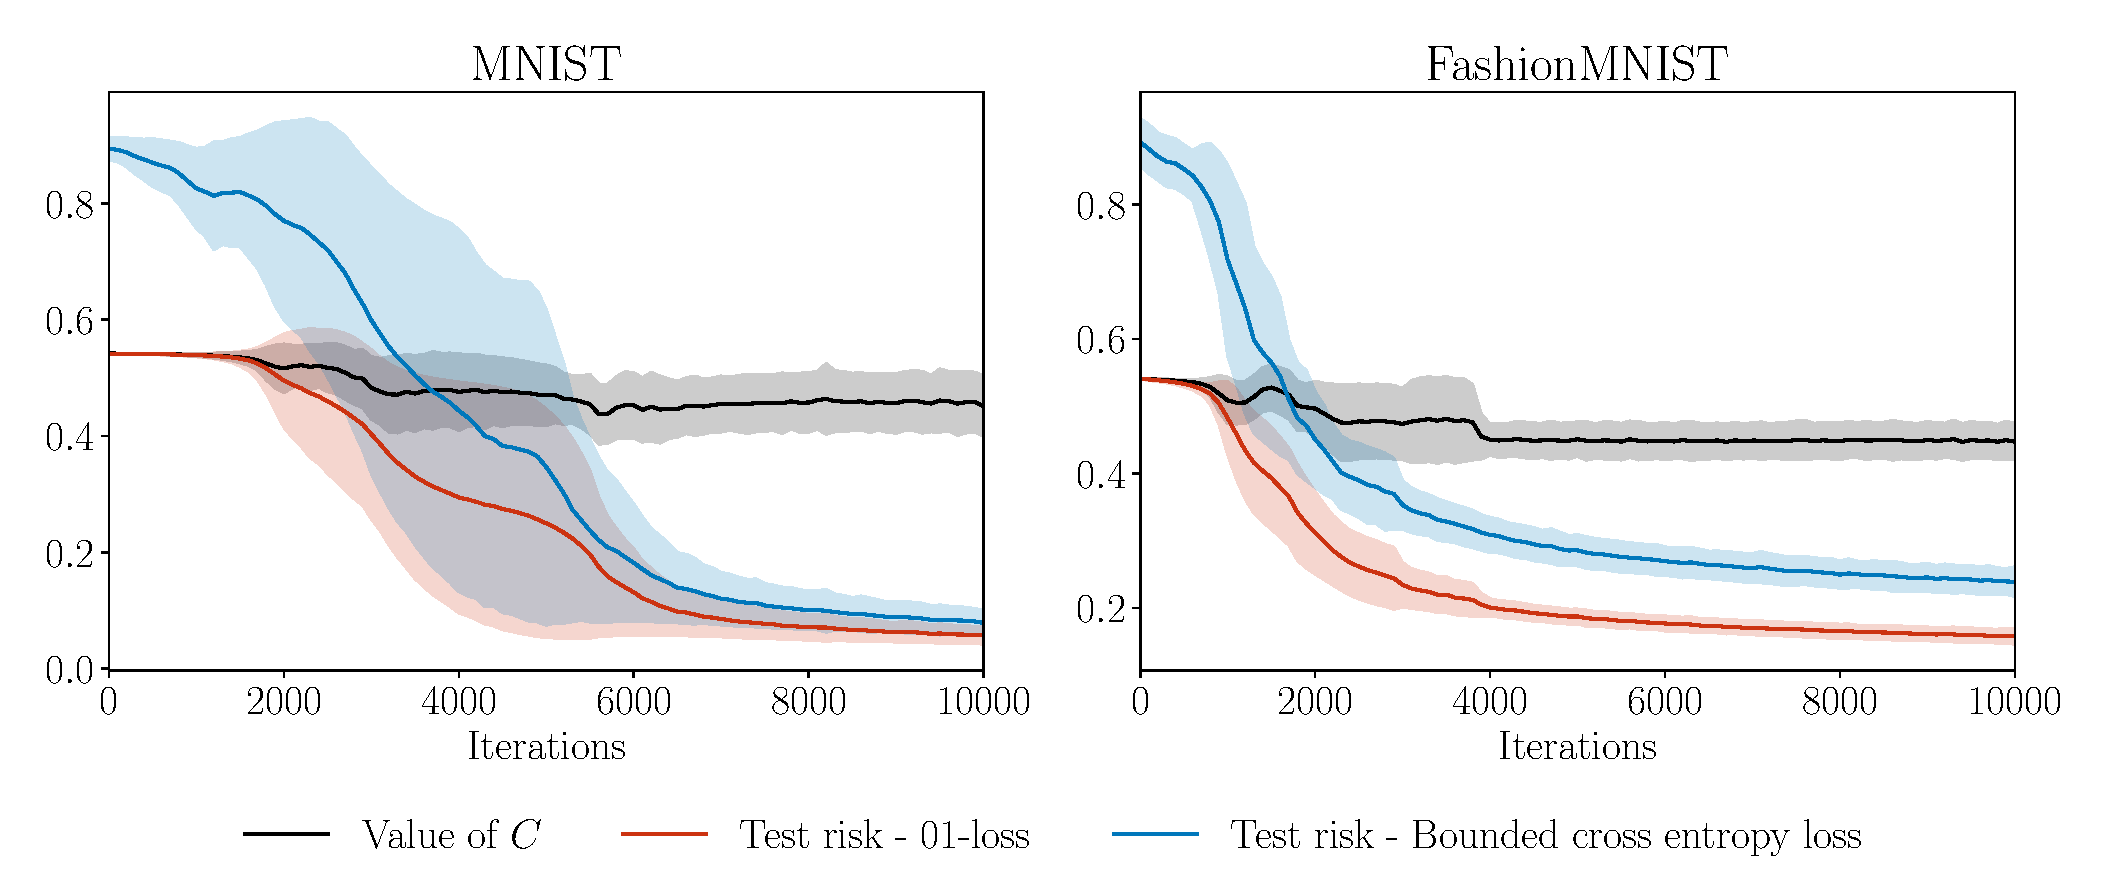
\includegraphics[width=1.0\linewidth]{chapter_4/figure.pdf}
    \caption{Evolution of the test risks (with the $01$-loss and the bounded cross-entropy loss) and the value of $C$ during the training phase.}
    \label{fig:expe}
\end{figure}

\paragraph{Empirical findings.}
\Cref{fig:expe} illustrates that, when neural networks are involved for two classification tasks, $\Q$ evolves during the optimisation process while maintaining the \texttt{QSB} property with constant $C<1$.
For both MNIST and FashionMNIST, the constant $C$ decreases from approximately 0.55 to 0.45. We deduce two things from this: \emph{(i)} the learning phase, while optimising $\hat{\Risk}_{\S_m}$ also gain in generalisation ability, shrinking the averaged loss on new data which is translated by a smaller $C$; and $(ii)$, having a data-free $\P$ (0 iteration) being \texttt{QSB} with $C<1$ suggests that the architecture of our neural network also has an influence on the $\texttt{QSB}$ assumption. As precised in \Cref{sec:poincare_gauss}, having $C<1$ attenuates the impact of the KL term, thus $\P$. This is desirable as it allows the optimiser to deeply explore the predictor space when $\P$ yields poor performances. We also note that the generalisation ability of $\Q$ on the training loss nearly matches the performance on the 0-1 loss for MNIST but is deteriorated for FashionMNIST, this invites to study more deeply the design of such surrogates in future work. 

\noindent{}Finally, the take-home message of this study is that the \texttt{QSB} assumption is verified for neural networks on MNIST. Such an empirical confirmation is crucial as it is required for our main result (Theorem \ref{th:poincaré_gauss}) and thus confirms that, for neural networks, reaching flat minima during the optimisation phase translates in increased generalisation ability.



\section{Conclusion}

This chapter showed that it is possible to exploit the benefits of a successful optimisation process to obtain faster rates, making a promising step forward a better understanding of deep neural networks, whose generalisation ability correlates well to flat minima. However, while we exploited potential benefits of optimisation process to make PAC-Bayes in line with optimisaiton, we still do not know whether an optimisation algorithm will reach a flat minima. This is somewhat unconsistent as optimisation processes are often supported by deterministic convergence guarantees. To fill this gap we show in \Cref{chap: wass-pb} that it is possible to incorporate directly optimisation guarantees onto PAC-Bayes bounds, making a supplementary step towards optimisation.
